\documentclass{article}
\usepackage{tikz}
\usetikzlibrary{graphs, graphs.standard, quotes, arrows.meta}

\begin{document}

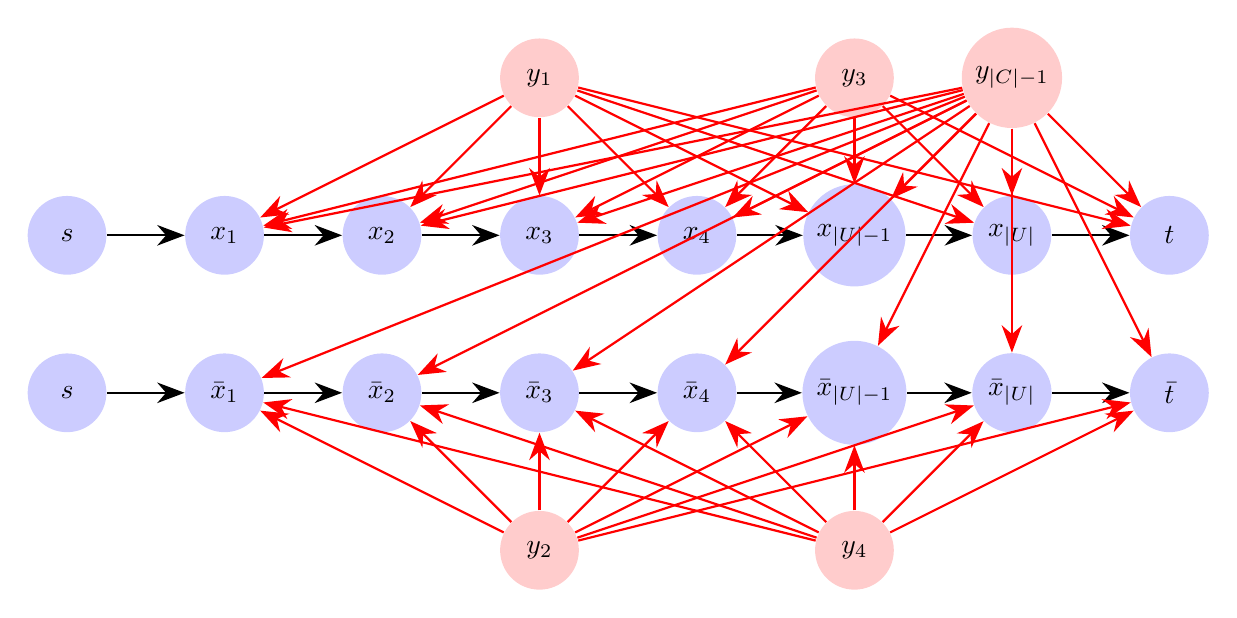
\begin{tikzpicture}[node distance=1cm]
    \tikzset{
        vertex/.style={circle, fill=blue!20, minimum size=1cm},
        edge/.style={-{Stealth[scale=1.5]}, thick},
        edge_red/.style={-{Stealth[scale=1.5]}, thick, red}
    }

    % Define nodes
    \node[vertex] (s) at (-3, 0) {$s$};
    \node[vertex] (x1) at (-1, 0) {$x_1$};
    \node[vertex] (x2) at (1, 0) {$x_2$};
    \node[vertex] (x3) at (3, 0) {$x_3$};
    \node[vertex] (x4) at (5, 0) {$x_4$};
    \node[vertex] (x5) at (7, 0) {$x_{|U|-1}$};
    \node[vertex] (x6) at (9, 0) {$x_{|U|}$};
    \node[vertex] (t) at (11, 0) {$t$};

    \node[vertex] (s') at (-3, -2) {$s$};
    \node[vertex] (x1') at (-1, -2) {$\bar{x}_1$};
    \node[vertex] (x2') at (1, -2) {$\bar{x}_2$};
    \node[vertex] (x3') at (3, -2) {$\bar{x}_3$};
    \node[vertex] (x4') at (5, -2) {$\bar{x}_4$};
    \node[vertex] (x5') at (7, -2) {$\bar{x}_{|U|-1}$};
    \node[vertex] (x6') at (9, -2) {$\bar{x}_{|U|}$};
    \node[vertex] (t') at (11, -2) {$\bar{t}$};

    \node[vertex, fill=red!20] (y1) at (3, 2) {$y_1$};
    \node[vertex, fill=red!20] (y2) at (3, -4) {$y_2$};
    \node[vertex, fill=red!20] (y3) at (7, 2) {$y_3$};
    \node[vertex, fill=red!20] (y4) at (7, -4) {$y_4$};
    \node[vertex, fill=red!20] (yc) at (9, 2) {$y_{|C|-1}$};

    % Draw edges
    \draw[edge] (s) -- (x1);
    \draw[edge] (x1) -- (x2);
    \draw[edge] (x2) -- (x3);
    \draw[edge] (x3) -- (x4);
    \draw[edge] (x4) -- (x5);
    \draw[edge] (x5) -- (x6);
    \draw[edge] (x6) -- (t);

    \draw[edge] (s') -- (x1');
    \draw[edge] (x1') -- (x2');
    \draw[edge] (x2') -- (x3');
    \draw[edge] (x3') -- (x4');
    \draw[edge] (x4') -- (x5');
    \draw[edge] (x5') -- (x6');
    \draw[edge] (x6') -- (t');

    \draw[edge_red] (y1) -- (x1);
    \draw[edge_red] (y1) -- (x2);
    \draw[edge_red] (y1) -- (x3);
    \draw[edge_red] (y1) -- (x4);
    \draw[edge_red] (y1) -- (x5);
    \draw[edge_red] (y1) -- (x6);
    \draw[edge_red] (y1) -- (t);

    \draw[edge_red] (y2) -- (x1');
    \draw[edge_red] (y2) -- (x2');
    \draw[edge_red] (y2) -- (x3');
    \draw[edge_red] (y2) -- (x4');
    \draw[edge_red] (y2) -- (x5');
    \draw[edge_red] (y2) -- (x6');
    \draw[edge_red] (y2) -- (t');

    \draw[edge_red] (y3) -- (x1);
    \draw[edge_red] (y3) -- (x2);
    \draw[edge_red] (y3) -- (x3);
    \draw[edge_red] (y3) -- (x4);
    \draw[edge_red] (y3) -- (x5);
    \draw[edge_red] (y3) -- (x6);
    \draw[edge_red] (y3) -- (t);

    \draw[edge_red] (y4) -- (x1');
    \draw[edge_red] (y4) -- (x2');
    \draw[edge_red] (y4) -- (x3');
    \draw[edge_red] (y4) -- (x4');
    \draw[edge_red] (y4) -- (x5');
    \draw[edge_red] (y4) -- (x6');
    \draw[edge_red] (y4) -- (t');

    \draw[edge_red] (yc) -- (x1);
    \draw[edge_red] (yc) -- (x2);
    \draw[edge_red] (yc) -- (x3);
    \draw[edge_red] (yc) -- (x4);
    \draw[edge_red] (yc) -- (x5);
    \draw[edge_red] (yc) -- (x6);
    \draw[edge_red] (yc) -- (t);

    \draw[edge_red] (yc) -- (x1');
    \draw[edge_red] (yc) -- (x2');
    \draw[edge_red] (yc) -- (x3');
    \draw[edge_red] (yc) -- (x4');
    \draw[edge_red] (yc) -- (x5');
    \draw[edge_red] (yc) -- (x6');
    \draw[edge_red] (yc) -- (t');
\end{tikzpicture}

\end{document}